% ============================================================
%  RAPPORT — Introduction au Traitement de Données
%  « L'anatomie d'un grand café arabica »
%  MAM3 — Polytech Nice Sophia — 2025-2026
% ============================================================
\documentclass[12pt,a4paper]{article}

% ---- Packages ----
\usepackage[T1]{fontenc}
\usepackage[utf8]{inputenc}
\usepackage[french,english]{babel}
\usepackage{charter}
\usepackage[top=2.5cm,bottom=2.5cm,left=2.5cm,right=2.5cm]{geometry}
\usepackage{graphicx}
\usepackage{booktabs}
\usepackage{array}
\usepackage{xcolor}
\usepackage{colortbl}
\usepackage{amsmath,amssymb}
\usepackage{hyperref}
\usepackage{float}
\usepackage{subcaption}
\usepackage{enumitem}
\usepackage{titlesec}
\usepackage{fancyhdr}
\usepackage{microtype}
\usepackage{parskip}
\usepackage{mdframed}
\usepackage{tcolorbox}
\usepackage{wrapfig}
\usepackage{multirow}

% ---- Couleurs thème café ----
\definecolor{coffeebrown}{RGB}{74,44,42}
\definecolor{coffeemedium}{RGB}{123,79,46}
\definecolor{coffeecream}{RGB}{245,230,200}
\definecolor{coffeegold}{RGB}{212,168,67}
\definecolor{accentgreen}{RGB}{92,122,62}
\definecolor{lightgray}{RGB}{245,245,245}

% ---- Hyperref ----
\hypersetup{
  colorlinks=true,
  linkcolor=coffeebrown,
  citecolor=accentgreen,
  urlcolor=coffeemedium,
  pdftitle={L'anatomie d'un grand café arabica},
  pdfauthor={Duburcq James - Lecureur Evrard - Waymel Clément}
}

% ---- En-têtes / Pieds de page ----
\pagestyle{fancy}
\fancyhf{}
\fancyhead[L]{\small\textcolor{coffeebrown}{\textit{Introduction au Traitement de Données - MAM3}}}
\fancyhead[R]{\small\textcolor{coffeebrown}{\thepage}}
\fancyfoot[C]{\small\textcolor{gray}{\textit{Duburcq James - Lecureur Evrard - Waymel Clément}}}
\renewcommand{\headrulewidth}{0.4pt}
\renewcommand{\headrule}{\hbox to\headwidth{\color{coffeebrown}\leaders\hrule height \headrulewidth\hfill}}

% ---- Titres de section ----
\titleformat{\section}
  {\Large\bfseries\color{coffeebrown}}
  {\thesection.}{0.5em}{}[\vspace{2pt}\color{coffeegold}\hrule height 1.5pt\vspace{4pt}]

\titleformat{\subsection}
  {\large\bfseries\color{coffeemedium}}
  {\thesubsection.}{0.5em}{}

\titleformat{\subsubsection}
  {\normalsize\bfseries\color{accentgreen}}
  {\thesubsubsection.}{0.5em}{}

% ---- Boîtes de mise en valeur ----
\tcbuselibrary{skins,breakable}
\newtcolorbox{insight}{
  enhanced,colback=coffeecream,colframe=coffeebrown,
  fonttitle=\bfseries\color{coffeebrown},
  title=Insight clé,arc=4pt,boxrule=1pt,
  left=6pt,right=6pt,top=4pt,bottom=4pt
}
\newtcolorbox{methode}{
  enhanced,colback=lightgray,colframe=accentgreen,
  fonttitle=\bfseries\color{accentgreen},
  title=Méthode,arc=4pt,boxrule=1pt,
  left=6pt,right=6pt,top=4pt,bottom=4pt
}

% ============================================================
\begin{document}
% ============================================================

% ---- Page de titre ----
\begin{titlepage}
\begin{center}
\vspace*{1cm}
{\color{coffeebrown}\rule{\linewidth}{2pt}}\\[0.4cm]
{\Huge\bfseries\color{coffeebrown} L'anatomie d'un grand café arabica}\\[0.3cm]
{\Large\color{coffeemedium}\textit{Quels critères définissent objectivement un café d'exception ?}}\\[0.4cm]
{\color{coffeebrown}\rule{\linewidth}{2pt}}\\[1.5cm]

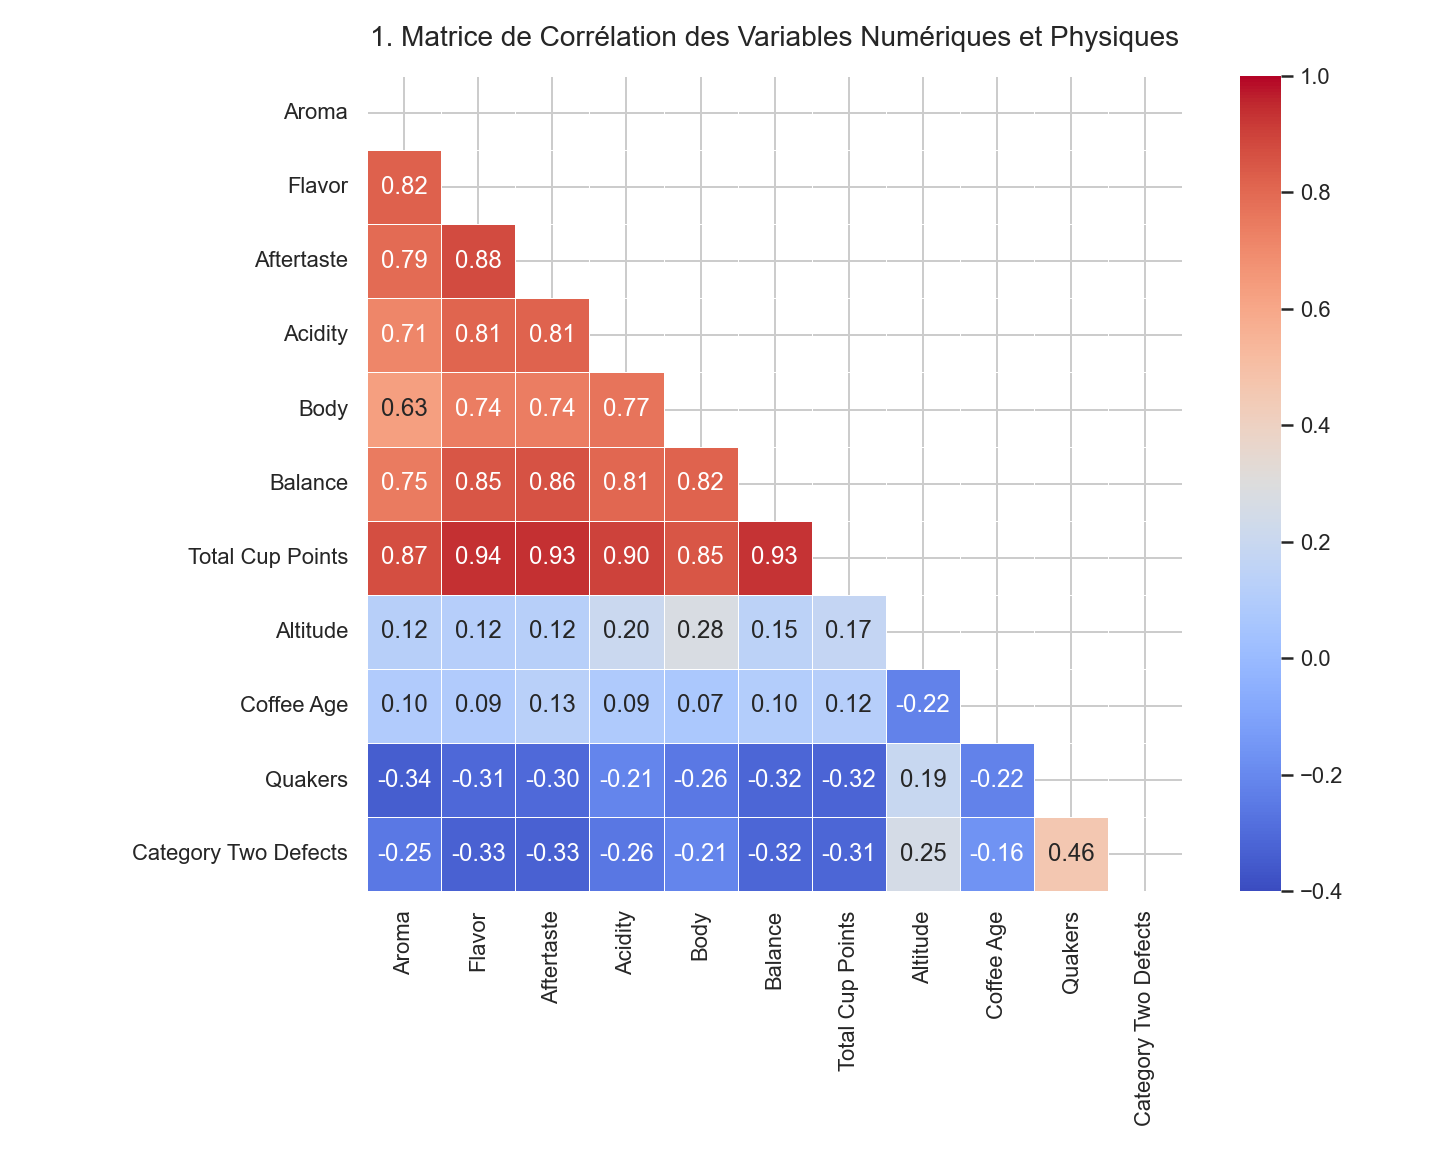
\includegraphics[width=0.55\linewidth]{figures/1_Matrice_de_correlation.png}\\[1cm]

\begin{tabular}{rl}
\textbf{\color{coffeebrown}Cours :} & Introduction au Traitement de Données\\
\textbf{\color{coffeebrown}Formation :} & Mathématiques Appliquées et Modélisation\\
\textbf{\color{coffeebrown}Établissement :} & Polytech Nice Sophia\\
\textbf{\color{coffeebrown}Dataset :} & CQI Arabica Coffee Quality Dataset (Kaggle)\\
\textbf{\color{coffeebrown}Dépôt Git :} & \href{https://github.com/evrardlecureur/TraitementDOnn-esMAM3}{TraitementDOnn-esMAM3}
\end{tabular}\\[2cm]

\end{center}
\end{titlepage}

% ---- Table des matières ----
\tableofcontents
\newpage

% ============================================================
\section{Business Goal — Le café, un objet de science}
% ============================================================

\subsection{Contexte}

Le café est l'une des boissons les plus consommées au monde, avec plus de 2,5 milliards de tasses
bues chaque jour. Pourtant, la frontière entre un café ordinaire et un café d'exception
reste souvent floue pour le consommateur. Pour les professionnels du secteur ( torréfacteurs,
importateurs, baristas ) cette question est au cœur de décisions économiques majeures.

Le \textbf{Coffee Quality Institute (CQI)} propose un protocole d'évaluation sensorielle
rigoureux, le cupping score, qui décompose la qualité d'un café en huit critères objectifs,
chacun noté de 6 à 10. Le score total (\textit{Total Cup Points}) est la somme de ces sous-scores.
Un café atteignant 80 points ou plus est qualifié de Specialty Coffee - la crème de la crème.


\begin{insight}
  Quels sont les facteurs ( sensoriels, géographiques, variétaux et agronomiques ) qui permettent de prédire et d'expliquer la qualité d'un café arabica noté par le CQI ?
\end{insight}


\subsection{Utilité du dataset}

Le dataset \texttt{df\_arabica\_clean.csv} (source : Kaggle, CQI) regroupe \textbf{207 échantillons}
de cafés arabica certifiés, notés entre 2021 et 2023, provenant de \textbf{23 pays}.
Il constitue une source idéale pour répondre à notre question car :
\begin{itemize}[noitemsep]
  \item Les notes sensorielles sont \textbf{standardisées} par des juges certifiés.
  \item Il couvre une grande diversité géographique,variétale et de méthodes de traitement.
  \item Il comprend à la fois des variables continues et des variables catégorielles.
\end{itemize}


% ============================================================
\section{Gestion d'équipe}
% ============================================================

\subsection{Organisation du travail}


Le travail a été organisé en phases successives.

\begin{center}
\begin{tabular}{@{}lll@{}}
\toprule
\rowcolor{coffeecream}
\textbf{Phase} & \textbf{Tâche principale} & \textbf{Date} \\
\midrule
1 & Choix du dataset, formulation de la question & 01/06 \\
2 & Nettoyage et exploration & 01/06 \\
3 & Visualisation et storytelling & 02/06 \\
4 & Feature engineering, régression & 02-03/06 \\
5 & Rédaction du rapport, préparation des slides & 04/06 \\
6 & Soutenance orale & 05/06 \\
\bottomrule
\end{tabular}
\end{center}

\subsection{Répartition des rôles}
 
Chaque membre a contribué à l'ensemble des phases du projet, avec des responsabilités principales
différenciées pour assurer une progression parallèle efficace.
 
\begin{center}
\begin{tabular}{@{}lccc@{}}
\toprule
\rowcolor{coffeecream}
\textbf{Tâche} & \textbf{Clément} & \textbf{Evrard} & \textbf{James} \\
\midrule
Choix du dataset et formulation de la question  & Contributeur & \textbf{Principal} & Contributeur \\
Nettoyage des données              & Contributeur & Contributeur & \textbf{Principal} \\
Exploration statistique                   & Contributeur & -- & \textbf{Principal} \\
Visualisation (figures 1-4)                    & \textbf{Principal} & Contributeur & Contributeur \\
Visualisation (figures 5-8)                    & Contributeur & -- & \textbf{Principal} \\
Feature engineering                             & \textbf{Principal} & Contributeur & Contributeur \\
Régression linéaire                             & Contributeur & -- & \textbf{Principal} \\
Rédaction du rapport                            & \textbf{Principal} & Contributeur & -- \\
Préparation des slides                          & -- & Contributeur & \textbf{Principal} \\
\bottomrule
\end{tabular}
\end{center}


% ============================================================
\section{Description des données}
% ============================================================

\subsection{Vue d'ensemble}

Le dataset contient 207 lignes et 41 colonnes, couvrant trois familles de variables :

\begin{center}
\begin{tabular}{@{}lll@{}}
\toprule
\rowcolor{coffeecream}
\textbf{Famille} & \textbf{Variables clés} & \textbf{Type} \\
\midrule
\textbf{Identité} & Pays, Région, Ferme, Variété, Propriétaire & Catégorielle / texte \\
\textbf{Agronomique} & Altitude, Méthode de traitement, Couleur, Humidité & Numérique / catég. \\
\textbf{Sensorielle} & Aroma, Flavor, Aftertaste, Acidity, Body, Balance, & Numérique [6--10] \\
& Uniformity, Clean Cup, Sweetness, Overall, Total Cup & \\
\textbf{Défauts} & Category One Defects, Category Two Defects, Quakers & Entier \\
\bottomrule
\end{tabular}
\end{center}

\subsection{Statistiques descriptives des critères sensoriels}

\begin{center}
\begin{tabular}{@{}lrrrrr@{}}
\toprule
\rowcolor{coffeecream}
\textbf{Critère} & \textbf{Min} & \textbf{Médiane} & \textbf{Moyenne} & \textbf{Max} \\
\midrule
Aroma        & 6.50 & 7.67 & 7.72 & 8.58 \\
Flavor       & 6.75 & 7.75 & 7.74 & 8.50 \\
Aftertaste   & 6.67 & 7.58 & 7.60 & 8.42 \\
Acidity      & 6.83 & 7.67 & 7.69 & 8.58 \\
Body         & 6.83 & 7.67 & 7.64 & 8.25 \\
Balance      & 6.67 & 7.67 & 7.64 & 8.42 \\
\midrule
\textbf{Total Cup Points} & 78.00 & 83.75 & 83.71 & 89.33 \\
\bottomrule
\end{tabular}
\end{center}

\paragraph{Note :} Les critères \textit{Uniformity}, \textit{Clean Cup} et \textit{Sweetness}
présentent des variances quasi nulles (presque tous égaux à 10 dans ce dataset), ce qui
explique leur faible pouvoir prédictif.

\subsection{Nettoyage}

\begin{itemize}[noitemsep]
  \item L'altitude est fournie comme texte libre ; elle a été convertie en numérique
        (\texttt{pd.to\_numeric(  , errors=`coerce')}), aboutissant à 153 valeurs valides sur 207.
  \item Les méthodes de traitement rares ont été regroupées en une catégorie
        « Autres » pour les analyses comparatives.
  \item La couleur des grains présente des incohérences typographiques (\textit{yellow green}
        vs \textit{yellow-green}), un nettoyage a été appliqué.
  \item Aucune ligne n'a été supprimée pour les analyses sensorielles (207 valeurs complètes).
\end{itemize}

% ============================================================
\section{Visualisation des données}
% ============================================================

\subsection{Corrélations entre les critères sensoriels}

\begin{figure}[H]
  \centering
  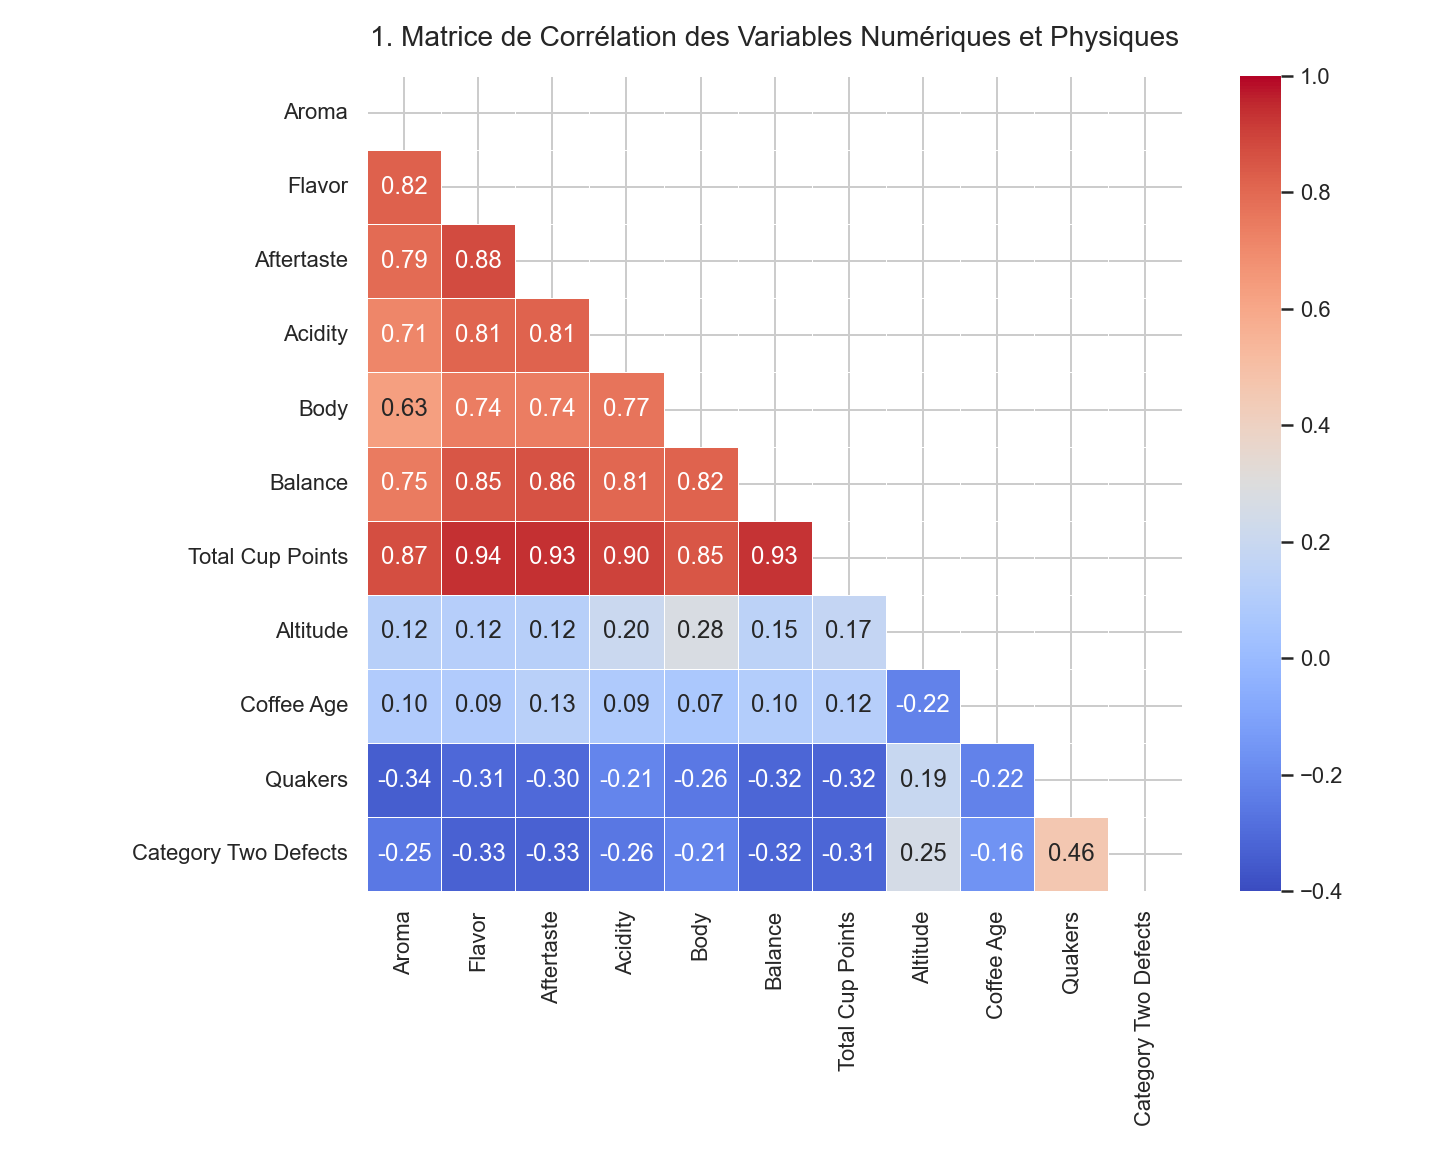
\includegraphics[width=0.72\textwidth]{figures/1_Matrice_de_correlation.png}
  \caption{Corrélogramme triangulaire inférieur des huit critères sensoriels (n\,=\,207).
           Les couleurs chaudes indiquent une forte corrélation positive.}
  \label{fig:corr}
\end{figure}

La figure~\ref{fig:corr} révèle que tous les critères sensoriels sont \textbf{fortement corrélés
entre eux} ($r > 0.70$ pour la plupart).
Les corrélations les plus élevées avec le \textit{Total Cup Points} sont :\textit{Flavor} ($r = 0.94$), \textit{Aftertaste} ($r = 0.93$)
et \textit{Balance} ($r = 0.93$).
L'\textit{Acidity} affiche également une corrélation très forte ($r = 0{,}90$), au même niveau que les
variables les plus discriminantes~: à elle seule, elle capture $r^2 \approx 0{,}80$ de la variance du score
global. Ce constat motive le choix de modélisation présenté dans la
sous-section suivante~: prédire l'acidité, c'est prédire $\sim$80\,\% de la
variance du \textit{Total Cup Points}.

\begin{insight}
  Un café arabica de qualité est un équilibre : aucun critère isolé ne suffit. La force du
  Flavor et de l'Aftertaste sont cependant les signaux les plus discriminants.
  L'\textit{Acidity} occupe une place à part~: corrélée à $0{,}90$ au score global, elle constitue un
  proxy statistiquement quasi parfait --- mais surtout un proxy \textbf{actionnable}, car elle est
  influencée par des variables physiques (altitude, terroir) que le producteur peut maîtriser.
\end{insight}

\subsection{Profil sensoriel selon la variété}

\begin{figure}[H]
  \centering
  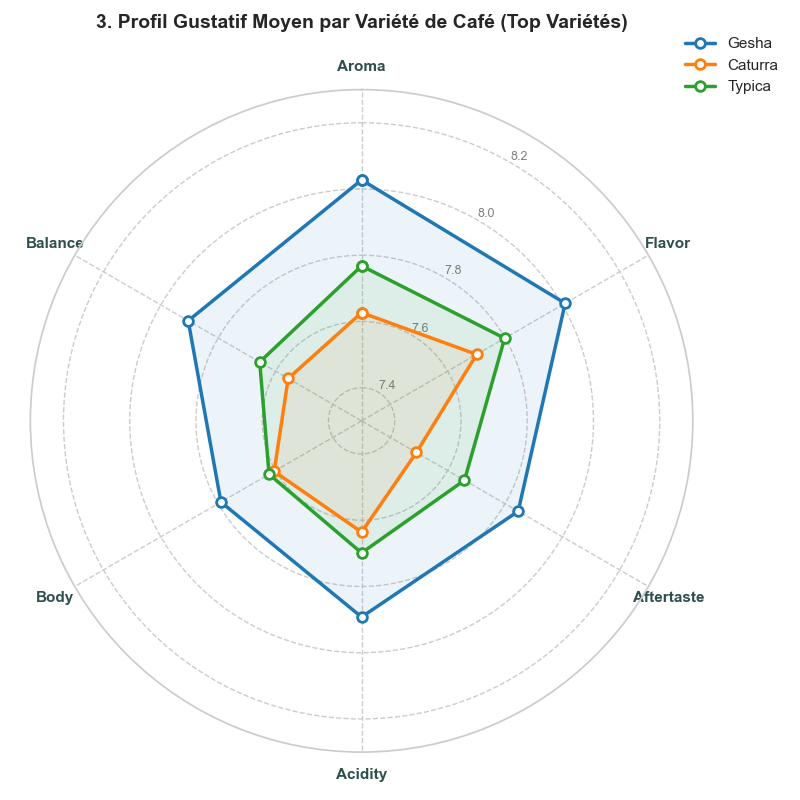
\includegraphics[width=0.62\textwidth]{figures/3_Graphique_radar.png}
  \caption{Diagramme radar des profils sensoriels moyens selon la variété.
           Les cafés « Gesha » se distinguent par un profil gustatif plus prononcé.}
  \label{fig:radar}
\end{figure}

La figure~\ref{fig:radar} compare trois variétés : Gesha, Caturra et Typica.
On observe que les cafés Caturra tendent à présenter un arrière-goût plus faible, tandis que les autres cafés sont plus équilibrés sur l'ensemble des critères.

\subsection{Scores par pays d'origine}

\begin{figure}[H]
  \centering
  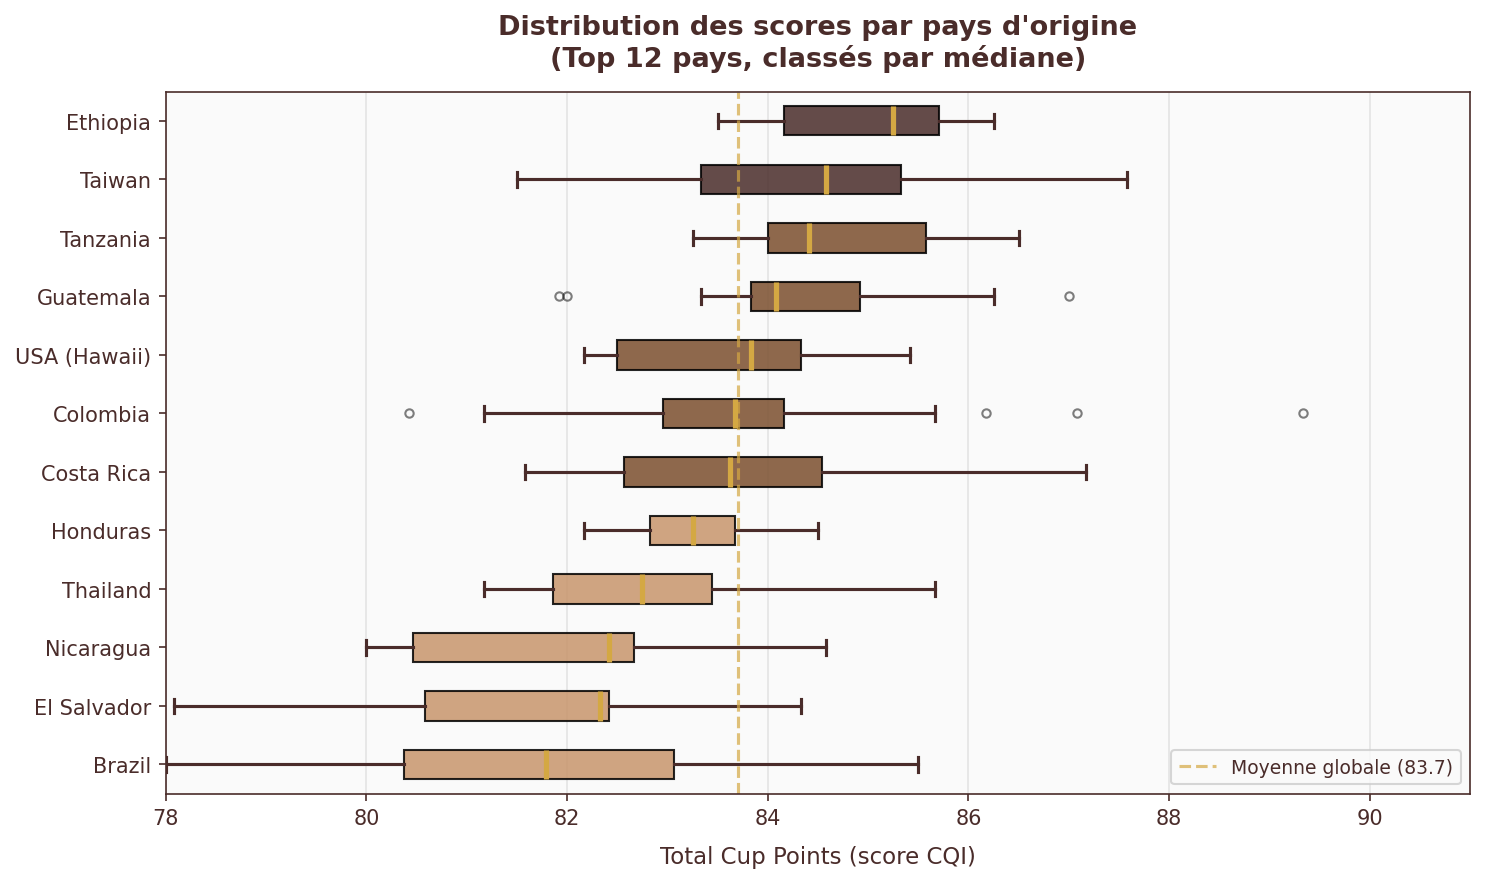
\includegraphics[width=0.90\textwidth]{figures/fig3_countries.png}
  \caption{Distribution du \textit{Total Cup Points} pour les 12 pays les plus représentés.
           Les boîtes à moustaches sont ordonnées par médiane croissante. La ligne pointillée
           indique la moyenne globale (83,7 pts).}
  \label{fig:pays}
\end{figure}

L'Éthiopie et la Tanzanie dominent le classement en termes de score médian
(respectivement 85,0 et 84,7 pts), loin devant le Brésil et El Salvador qui peinent à dépasser
82 pts en médiane. Taiwan, très représenté ($n=61$), affiche une médiane élevée (84,4 pts) avec une
grande dispersion, témoignant d'une filière dynamique mais hétérogène.

\subsection{Influence de l'altitude}
La corrélation brute altitude-score est modeste. Cependant, comme nous le verrons lors du Feature Engineering (Section 5), l'analyse par tranches d'altitude révèle un véritable effet de seuil : les cafés cultivés au-delà de 1800\,m obtiennent en moyenne 84,8 pts (moyenne des traitements), soit +1,3 pt par rapport aux cafés cultivés sous 1000\,m (83,5 pts).

% ============================================================
\section{Feature Engineering - Valoriser les signaux faibles}
% ============================================================

\subsection{Variables directement disponibles (features brutes)}

Les six critères sensoriels (Aroma, Flavor, Aftertaste, Acidity, Body, Balance) constituent des descripteurs de tasse essentiels. Cependant, comme mis en évidence lors de la phase de visualisation, ces notes souffrent d'une forte multicolinéarité ($r > 0.70$). Pour construire un modèle prédictif robuste et stable, utile aux acteurs de la filière (producteurs et négociants), il est nécessaire de déplacer le focus vers les variables physiques, environnementales et temporelles stables.

\subsection{Transformations stratégiques (Features construites)}

Afin d'enrichir nos modèles et de capturer des relations non-linéaires, quatre transformations majeures ont été conçues :

\begin{itemize}[noitemsep]
  \item Paliers d'Altitude : Afin de modéliser une segmentation climatique potentiellement non-linéaire, l'altitude brute a été discrétisée en 4 classes géographiques et thermiques majeures :
        \begin{itemize}
          \item Basses altitudes : $< 1200$\,m
          \item Altitudes intermédiaires : $1200\,\text{m} - 1500$\,m
          \item Hautes altitudes : $1500\,\text{m} - 1800$\,m
          \item Très hautes altitudes : $> 1800$\,m
        \end{itemize}
  \item Procédés Harmonisés : Les modes de préparation initiaux, trop fragmentés dans le jeu de données d'origine, ont été regroupés et harmonisés en 3 grandes familles technologiques homogènes : Washed/Wet, Natural/Dry et Pulped natural/honey.
  \item Macro-Régions : Pour stabiliser les prédictions face à la forte cardinalité des pays d'origine (23 pays), une variable de regroupement géographique a été créée autour de trois grands terroirs climatiques homogènes : Afrique, Amériques et Asie-Pacifique. Ce découpage capture les spécificités bioclimatiques de chaque continent sans diluer l'information dans une multitude de classes rares.
  \item Âge du Café (Facteur temporel) : Création d'une variable temporelle continue calculant le temps précis écoulé entre la date de récolte du lot de café et sa date d'expiration certifiée.
\end{itemize}

\subsection{Vérification de la pertinence des features construites}

\begin{figure}[H]
  \centering
  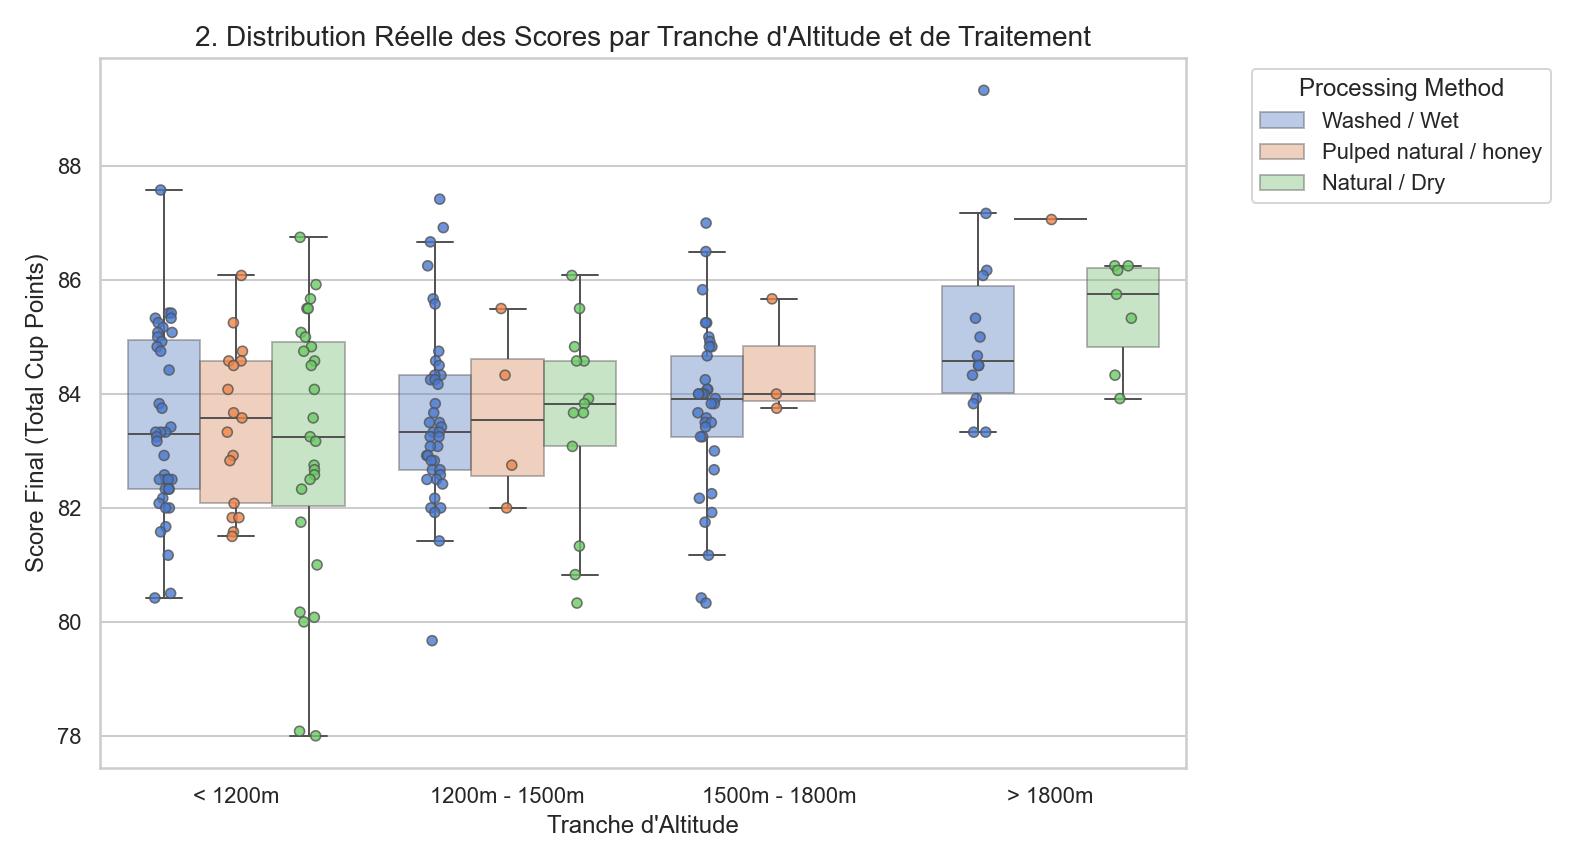
\includegraphics[width=0.88\textwidth]{figures/2_Distribution_scores_altitude.png}
  \caption{Distribution réelle des scores finaux selon les tranches d'altitude construites et les méthodes de traitement associées.}
  \label{fig:dist_features}
\end{figure}

L'analyse croisée de ces nouvelles variables (Figure~\ref{fig:dist_features}) valide notre intuition statistique. On observe un net effet de seuil lié à l'altitude : au-delà de 1800\,m, la moyenne des scores se stabilise à un niveau élevé (84,8 pts). De plus, à très haute altitude, les procédés Washed/Wet et Natural/Dry affichent des comportements plus réguliers, limitant la dispersion des notes vers le bas.
% ============================================================
\section{Modélisation}
% ============================================================

\subsection{Prédiction globale : l'Indice de Qualité Composite}

Afin d'anticiper la note \textit{Total Cup Points} ($Y$) avant les phases subjectives de dégustation, un modèle de régression linéaire multiple (Moindres Carrés Ordinaires) a été entraîné sur 10 variables exclusivement physiques, géographiques et temporelles : altitude, âge du lot, taux d'humidité, défauts de catégorie 1 et 2, grains Quakers, méthode de traitement, couleur du grain, pays de production et variété botanique (ces quatre dernières encodées en One-Hot).

\begin{figure}[H]
  \centering
  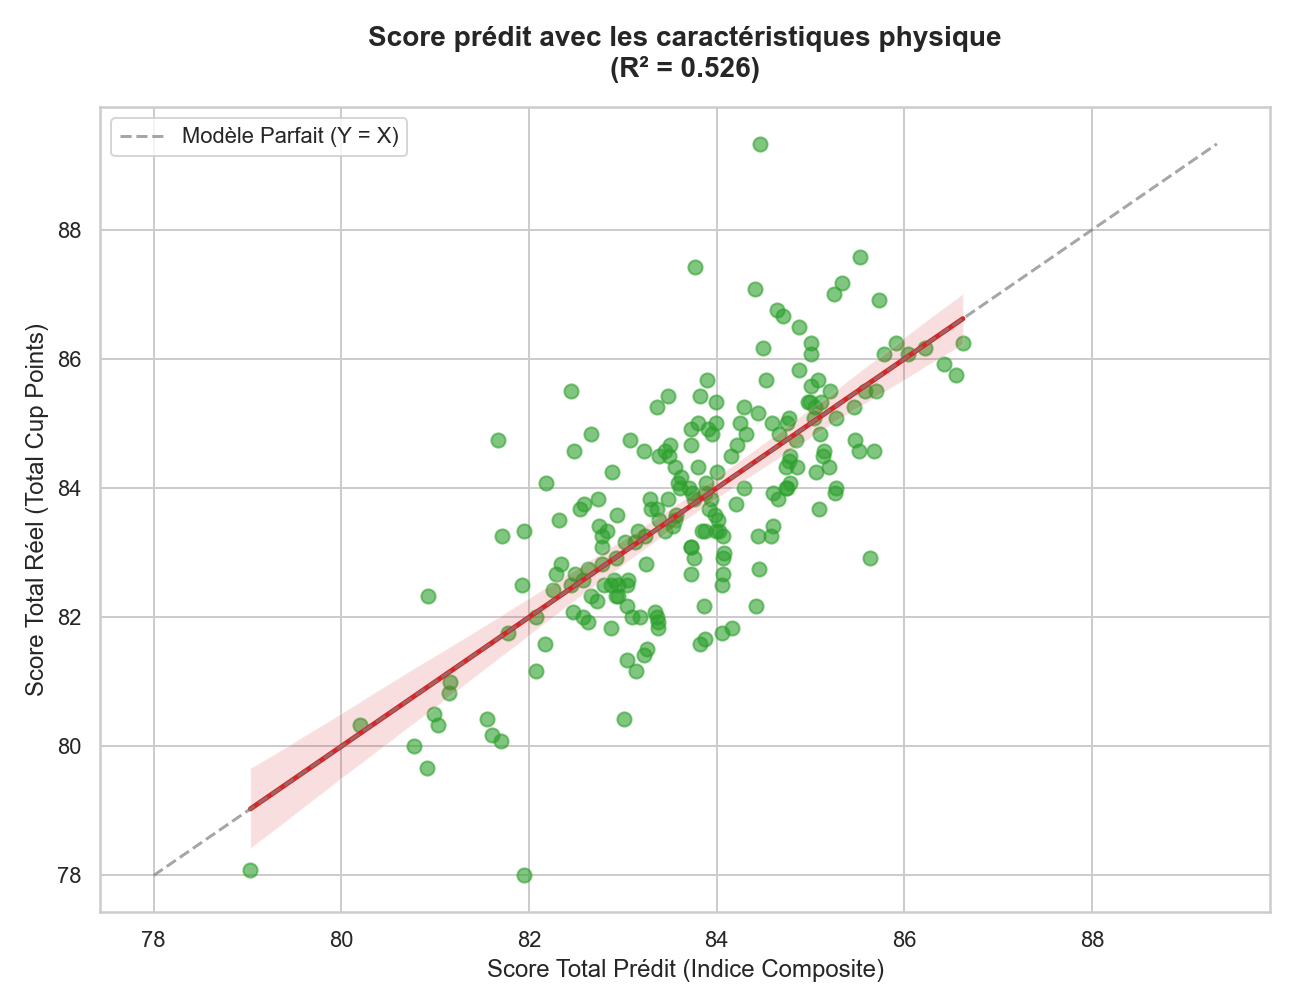
\includegraphics[width=0.85\textwidth]{figures/score_predit_caracteristiques_physiques.png}
  \caption{Confrontation entre le score composite prédit ($\widehat{Y}$) et la qualité réelle observée (\textit{Total Cup Points}).}
  \label{fig:modele_etendu}
\end{figure}

L'analyse des coefficients révèle que les défauts de catégorie 2 et les Quakers sont les principaux vecteurs de dépréciation du score, tandis que l'altitude agit positivement, en cohérence avec la littérature agronomique. L'âge du lot et l'humidité, bien que secondaires, décrivent l'état de conservation du café.

Comme l'illustre la Figure~\ref{fig:modele_etendu}, ce modèle atteint un coefficient de détermination \textbf{$R^2 = 0.526$}. Expliquer plus de la moitié de la variance d'une évaluation sensorielle humaine uniquement à partir de caractéristiques techniques mesurables constitue une performance solide pour un outil d'aide à la décision précoce.

\begin{insight}
  L'évaluation du potentiel d'un café de spécialité peut s'affranchir des phases de dégustation initiales : l'intégrité physique du lot et son contexte de culture fournissent une estimation fiable avant l'importation.
\end{insight}

\subsection{Acidity comme proxy du score global : effet de l'altitude selon la région}

\begin{insight}
\textbf{Pourquoi l'\textit{Acidity} et non le \textit{Total Cup Points} ?}
Le \textit{Total Cup Points} étant la somme de 10 sous-scores sensoriels, le
prédire directement reviendrait à régresser sur une variable composite dont
aucune composante n'est actionnable individuellement. La matrice de corrélation
(Figure~\ref{fig:corr}) montre que l'\textit{Acidity} est fortement corrélée au
score global ($r = 0{,}90$, $r^2 \approx 0{,}80$) : à elle seule, elle capture
80\,\% de la variance du \textit{Total Cup Points}. Étudier les déterminants de
l'acidité revient donc à étudier l'un des principaux déterminants du score
final --- avec l'avantage décisif que l'acidité, contrairement à \textit{Flavor}
ou \textit{Aftertaste}, est un critère objectivement mesurable sur le grain
vert, donc modélisable par des variables physiques (altitude, origine,
traitement). C'est précisément ce qu'illustre la
Figure~\ref{fig:proxy_acidite_tcp} : la relation linéaire est si serrée que la
plupart des points tombent dans la bande de confiance à 95\,\%.
\end{insight}

Au-delà de la prédiction globale, une seconde modélisation affine la
compréhension du lien entre terroir et profil aromatique. Un modèle
d'interaction linéaire a été ajusté pour prédire le sous-score \textit{Acidity}
en fonction de l'altitude, de la macro-région, et de leur produit croisé~:

\begin{equation}
\text{Acidity} \sim \text{Altitude} + \text{Macro-Région} + \text{Altitude} \times \text{Macro-Région}
\end{equation}

\begin{figure}[H]
  \centering
  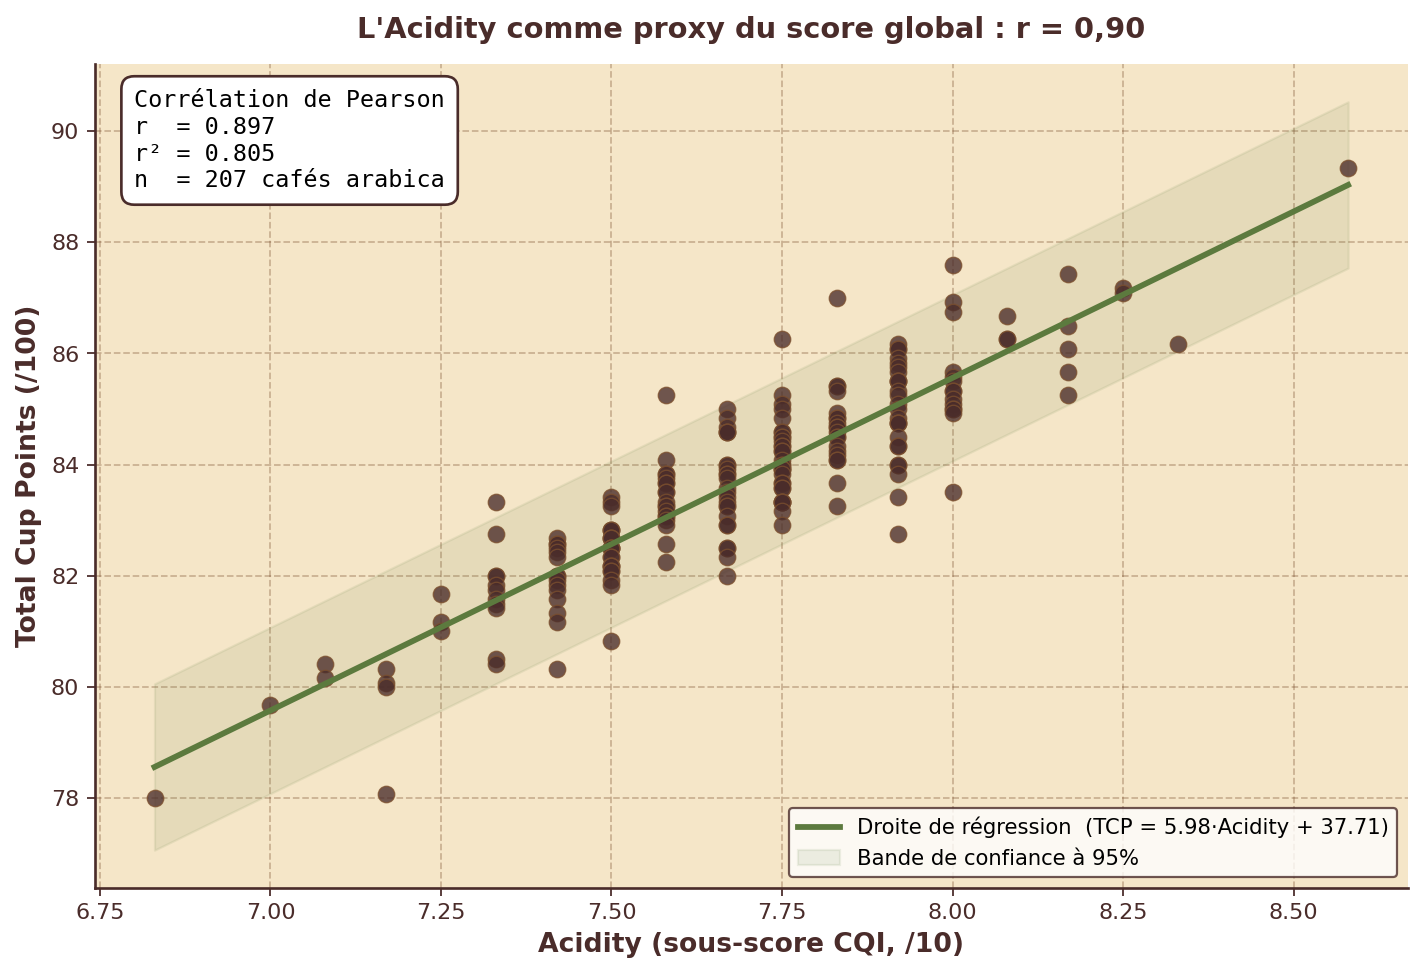
\includegraphics[width=0.80\textwidth]{figures/fig_acidity_vs_tcp.png}
  \caption{Justification empirique du choix de \textit{Acidity} comme cible~:
           la corrélation linéaire avec le \textit{Total Cup Points} est
           $r = 0{,}90$ ($r^2 = 0{,}80$, $n = 207$). La bande verte représente
           l'intervalle de confiance à 95\,\% de la droite de régression.}
  \label{fig:proxy_acidite_tcp}
\end{figure}

\begin{figure}[H]
  \centering
  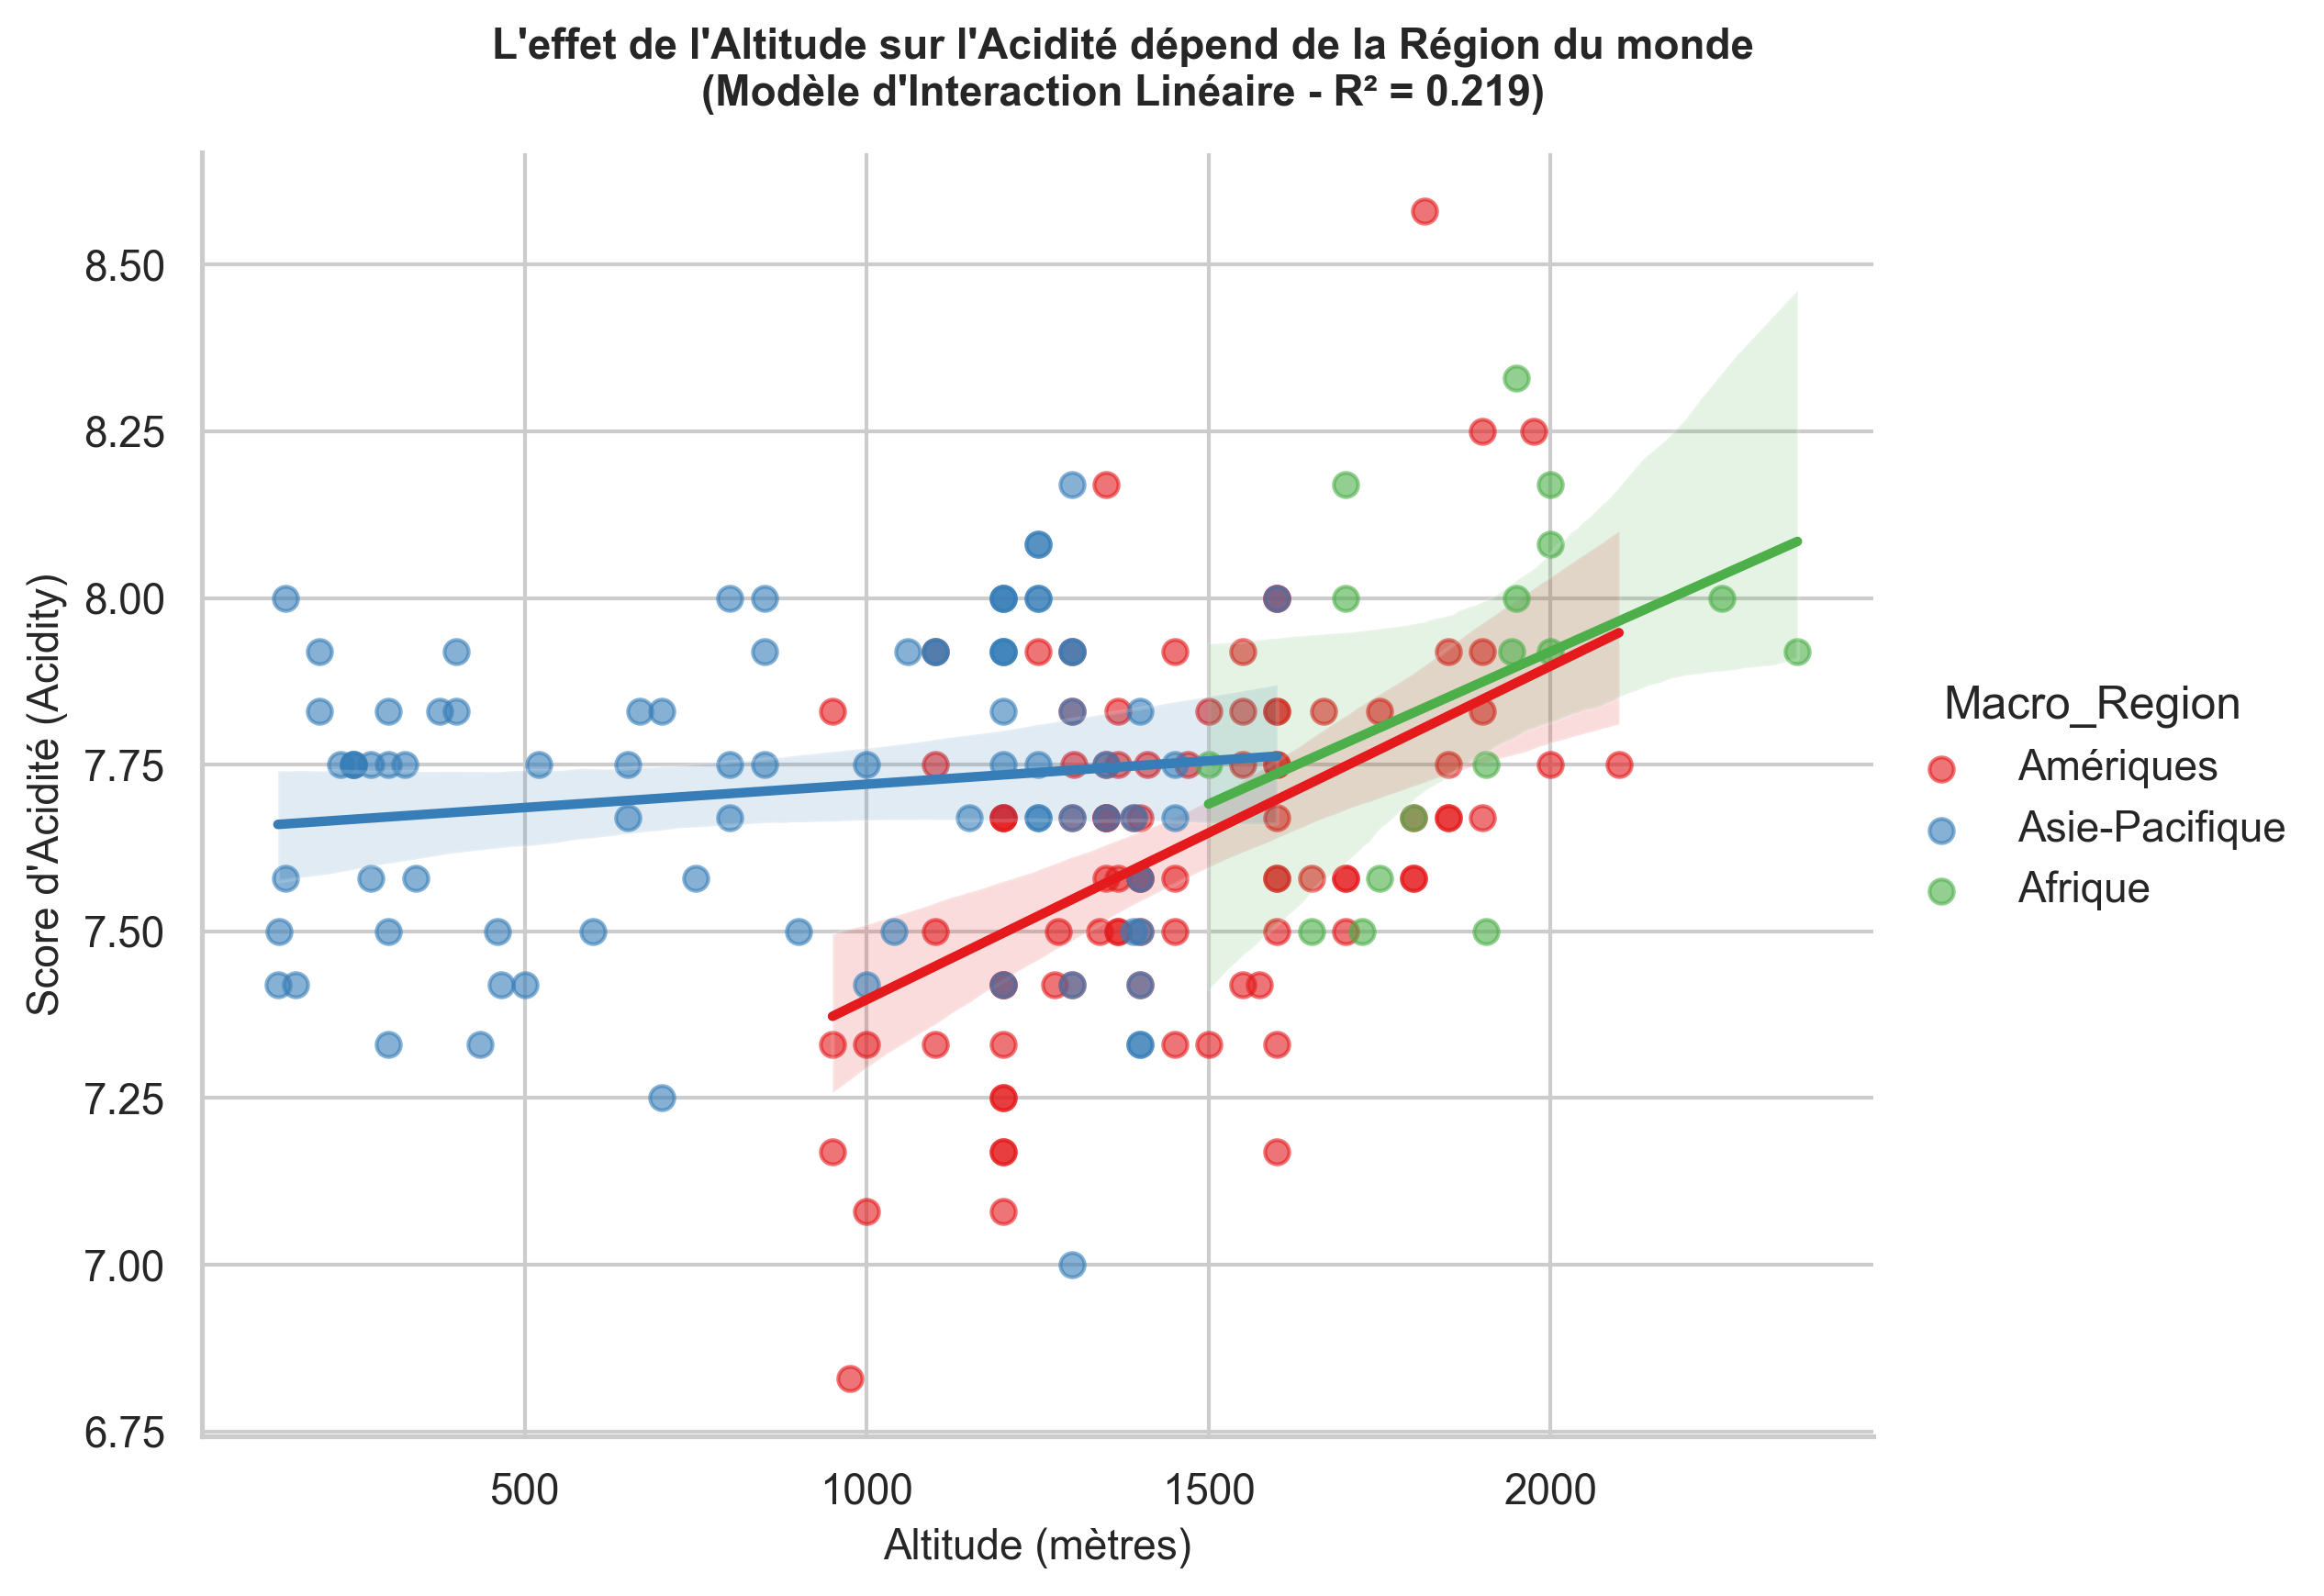
\includegraphics[width=0.85\textwidth]{figures/graphique_interaction_macro_regions.png}
  \caption{Effet de l'altitude sur l'acidité selon la macro-région de production. Les pentes hétérogènes montrent que l'altitude n'a pas le même impact selon le continent.}
  \label{fig:interaction_acidite}
\end{figure}

La Figure~\ref{fig:interaction_acidite} met en évidence une dissociation nette entre les trois macro-régions. En Afrique, l'acidité augmente sensiblement avec l'altitude, ce qui correspond aux conditions bioclimatiques des hauts plateaux est-africains. En Asie-Pacifique, la pente est quasi nulle : l'acidité reste stable quelle que soit l'altitude. Dans les Amériques, la tendance est intermédiaire. Ce résultat montre que la relation altitude--qualité, souvent présentée comme universelle, est en réalité conditionnée par le contexte climatique régional.

Le modèle atteint un $R^2 = 0.219$. Bien que modeste, cette valeur est cohérente avec la nature très locale et multifactorielle de l'acidité. L'apport clé de cette analyse est moins prédictif qu'\textbf{explicatif} : elle démontre que l'interaction géographie $\times$ altitude capte une information que ni l'altitude seule ni la région seule ne peuvent exprimer.
% ============================================================
\section{Conclusion}
% ============================================================

\subsection{Enseignements de l'analyse}

Notre analyse du dataset CQI Arabica apporte des réponses concrètes à la question
\textit{« Quels critères définissent objectivement un café d'exception ? »}, tout en s'affranchissant de la subjectivité de la dégustation :

\begin{enumerate}
  \item \textbf{La prédictibilité par l'agronomie et la physique :} Il est possible d'expliquer une grande partie de la variance de la note finale (jusqu'à $R^2 \approx 0.53$) en se basant strictement sur des critères vérifiables avant la torréfaction. 
  \item \textbf{L'importance vitale de l'intégrité physique :} Les défauts (notamment les Quakers et ceux de catégorie 2) appliquent une pénalité sévère et quasi-immédiate sur la note finale. Le tri visuel et physique reste la première barrière d'entrée vers la spécialité.
  \item \textbf{La prime au Terroir et à la Botanique :} L'origine géographique et la génétique (les variétés comme le \textit{Gesha} ou le \textit{Typica}) agissent comme d'importants "boosters" de score, offrant une prime naturelle à certains lots.
  \item \textbf{L'effet de l'altitude :} Une altitude élevée (notamment l'effet de seuil au-delà de 1800\,m) est statistiquement associée à des scores supérieurs, ce qui corrobore le principe agronomique d'une maturation ralentie des cerises.
  \item \textbf{L'interaction altitude--géographie :} L'analyse par macro-régions révèle que l'effet de l'altitude sur l'acidité n'est pas universel : il est fort en Afrique, quasi inexistant en Asie-Pacifique et intermédiaire dans les Amériques. Cette dissociation remet en question la vision d'un lien altitude--qualité uniforme et souligne l'importance des conditions bioclimatiques locales. Comme l'acidité capte à elle seule $\sim$80\,\% de la variance du \textit{Total Cup Points} ($r = 0{,}90$), comprendre ses déterminants territoriaux revient à comprendre l'un des principaux leviers objectifs de la qualité globale~: la pente «~altitude--qualité~» que l'on croyait universelle est en fait une mosaïque de comportements régionaux.
\end{enumerate}

\subsection{Limites et perspectives}

\begin{itemize}[noitemsep]
  \item \textbf{Taille de l'échantillon :} Le dataset ne compte que 207 observations, ce qui limite la robustesse statistique, notamment pour l'analyse des origines rares à de très hautes altitudes.
  \item \textbf{Données climatiques manquantes :} Pour aller plus loin dans l'analyse du terroir, il serait pertinent d'intégrer des données macro-économiques et météorologiques exogènes telles que la pluviométrie et les températures régionales annuelles.
  \item \textbf{Impact économique :} Une extension naturelle consisterait à croiser ces scores avec les données de prix du marché pour chiffrer directement la perte ou le gain de valeur commerciale lié aux défauts physiques.
  \item \textbf{Modélisation avancée :} Le passage à des modèles non-linéaires (Random Forest, XGBoost) ou intégrant une régularisation (Ridge/Lasso) permettrait d'améliorer la prédiction tout en gérant mieux les variables colinéaires.
\end{itemize}


\end{document}
